\begin{figure}[tb]
	\hfill
	\begin{subfigure}[c]{0.4\linewidth}
		\centering
		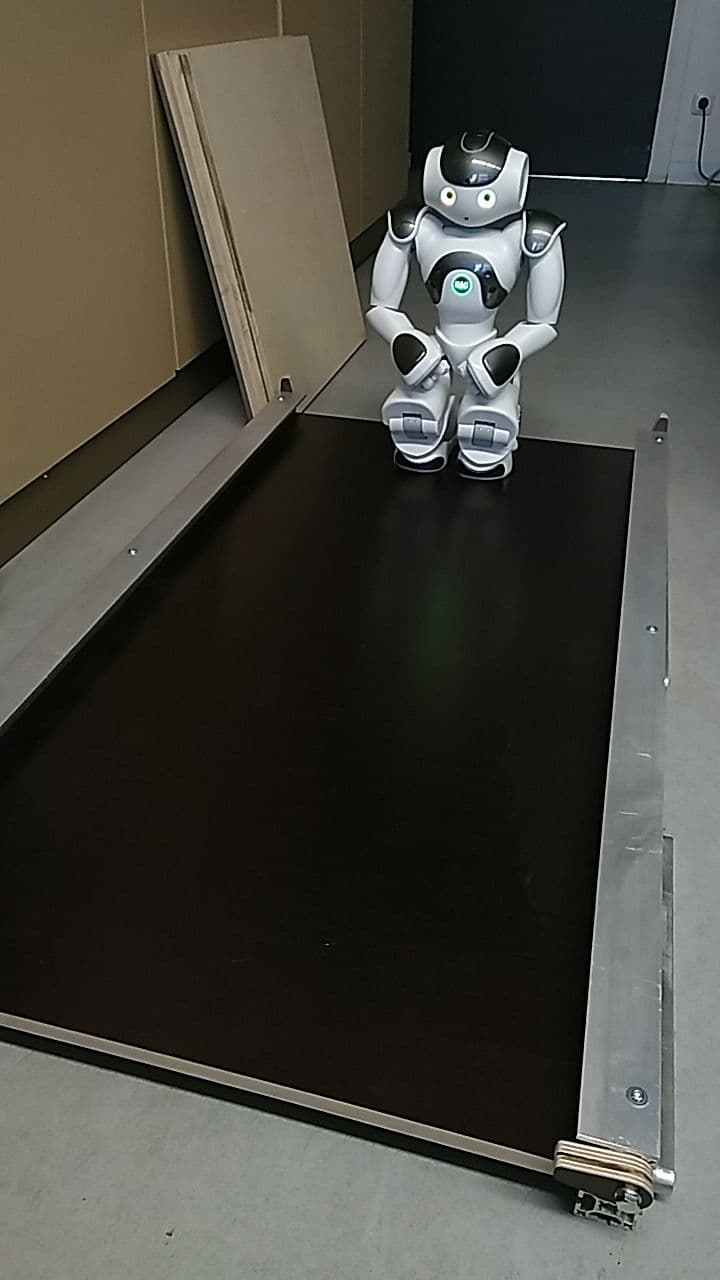
\includegraphics[width=\linewidth]{Bilder/NAO_auf_Rampe2.jpg}
	\end{subfigure}
	\hfill
	\begin{subfigure}[c]{0.4315\linewidth}
		\centering
		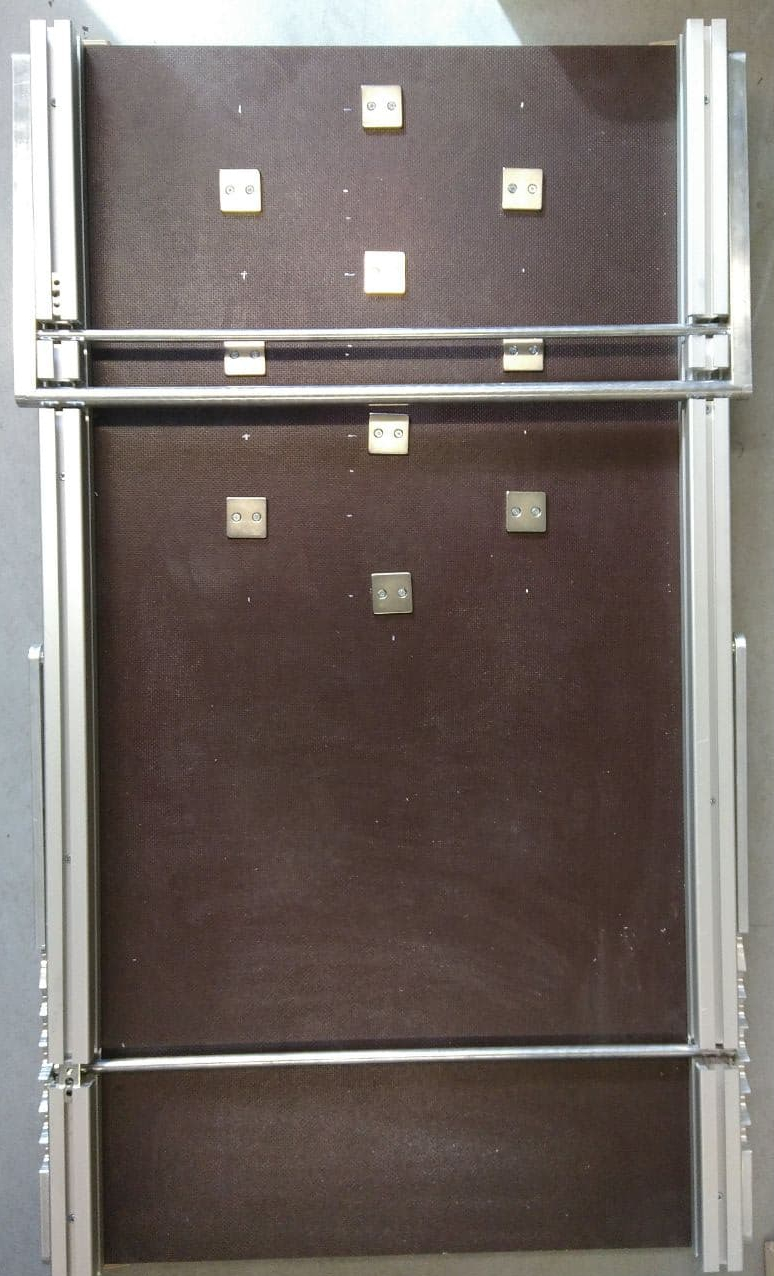
\includegraphics[width=\linewidth]{Bilder/magneten_an_rampe1_geschnitten.jpg}
	\end{subfigure}
	\hfill
	\caption{}
	\label{nao_und_rampe}
\end{figure}

\begin{figure}[tb]
	\hfill
	\begin{subfigure}[c]{0.3\linewidth}
		\centering
		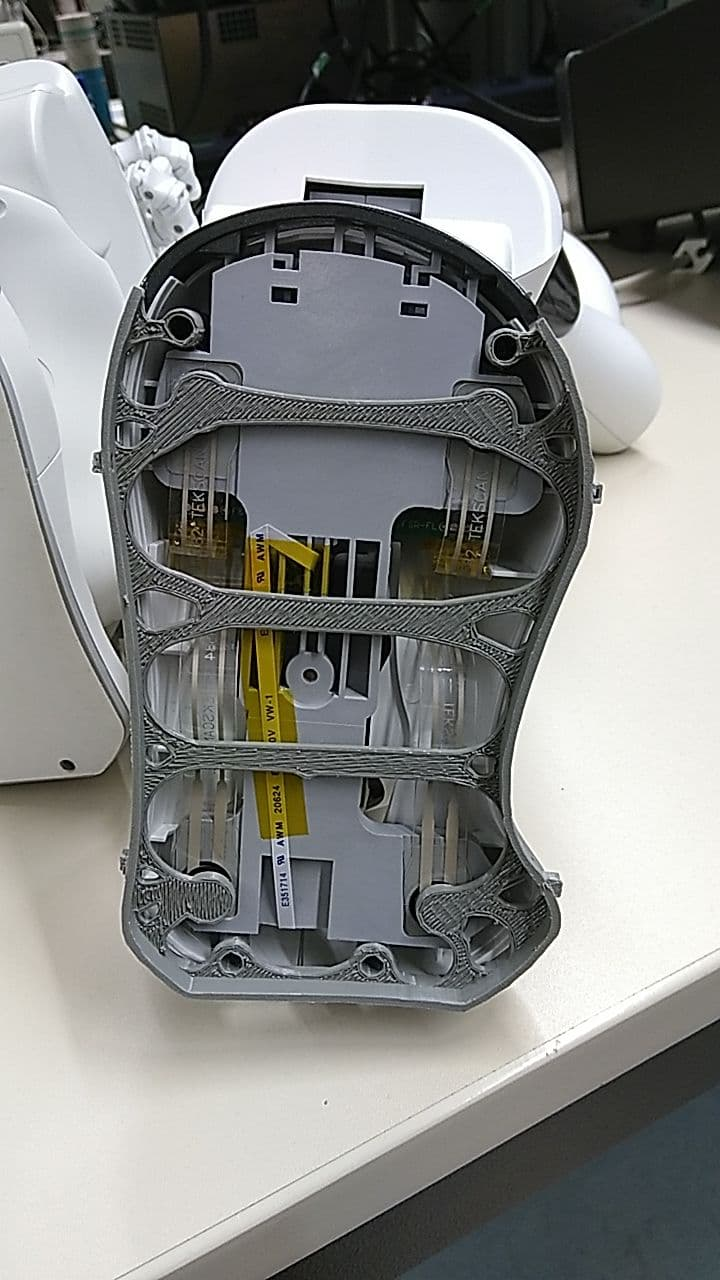
\includegraphics[width=\linewidth]{Bilder/Schuh_an_NAO_ohne_Sohle.jpg}
	\end{subfigure}
	\hfill
	\begin{subfigure}[c]{0.6\linewidth}
		\centering
		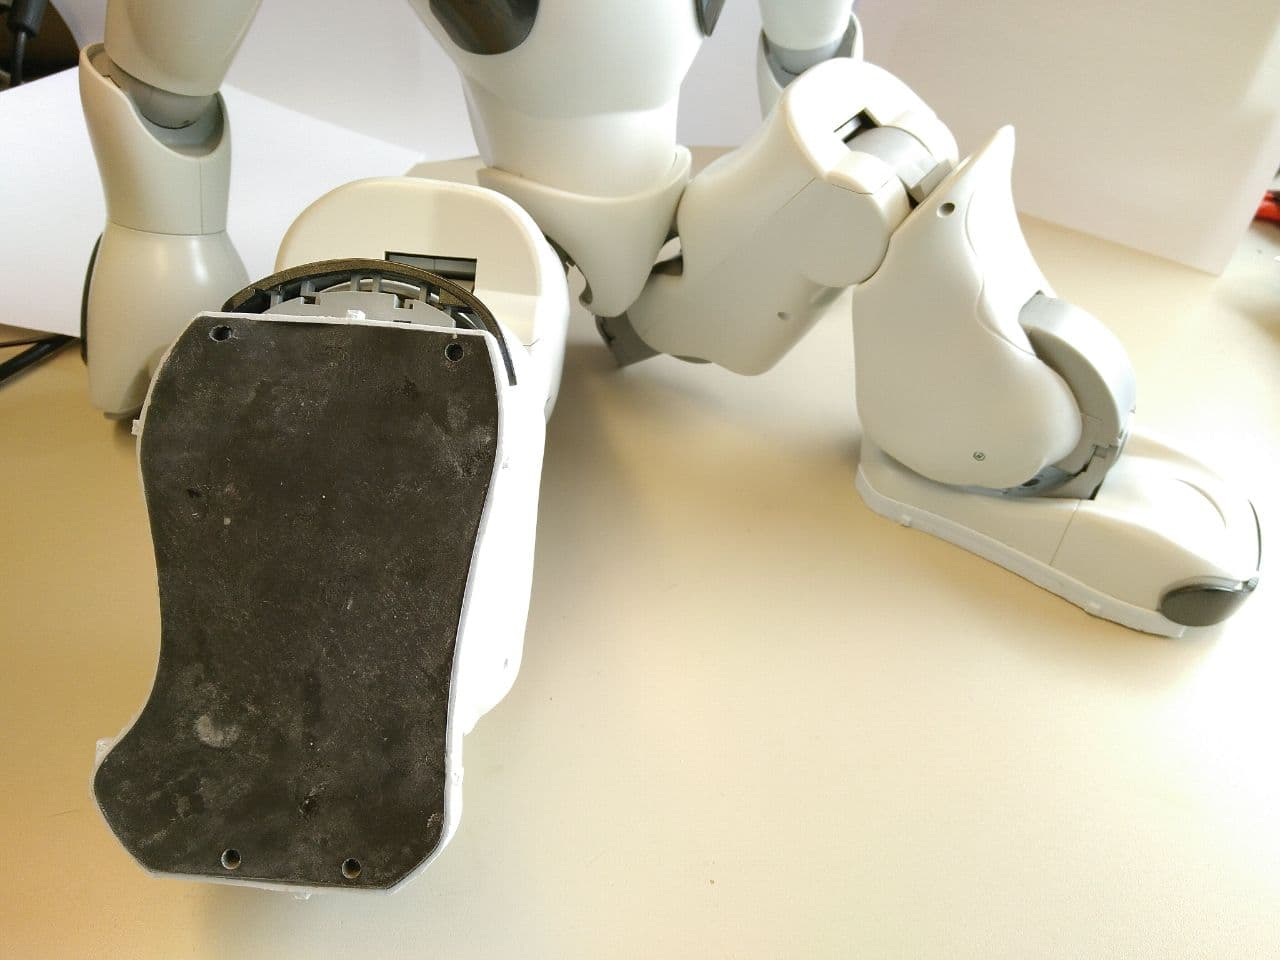
\includegraphics[width=\linewidth]{Bilder/Schuh_an_NAO_mit_Sohle.jpg}
	\end{subfigure}
	\hfill
	\caption{}
	\label{nao_mit_schuhen}
\end{figure}